\section{Motivație}

Anual se produc peste 8 000 de accidente rutiere grave în România, din care rezultă peste 7 000 de răniți grav și peste 2 000 de persoane decedate. Principalul motiv al tuturor acestor incidente, este de departe reprezentat de erorile umane, de la neatenție sau lipsa de experiență până la oboseală.
\begin{figure}[!h]
	\centering
	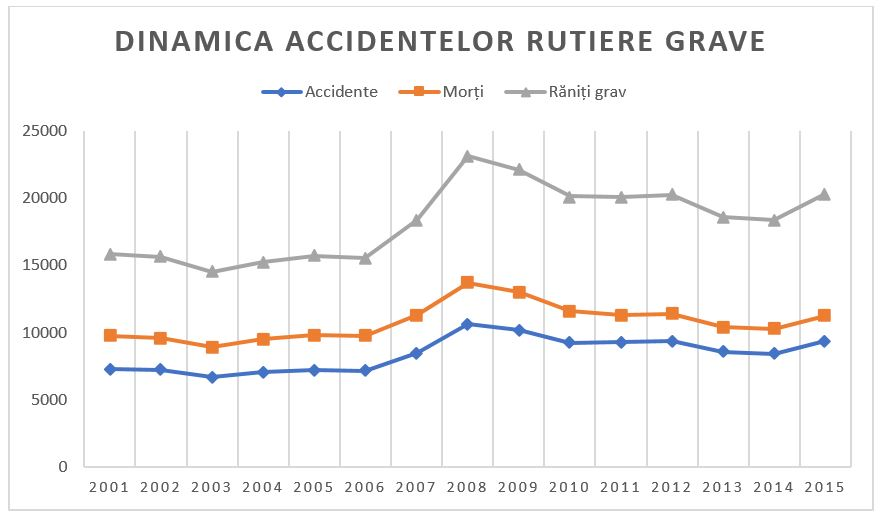
\includegraphics[max width=15cm,max height=15cm,keepaspectratio]{img_1_1}
	\caption[Dinamica accidente rutiere]{Dinamica accidentelor grave produse în România în perioada 2001 - 2015. Statistică preluată din \hyperlink{Dinamicaaccidentelorrutiere}{[8]}.}
\end{figure} 

Însă, o foarte mare parte a erorilor ce cauzează producerea de accidente rutiere pot fi evitate cu ajutorul sistemelor dotate cu inteligență artificială. Sisteme ce pot fi de la cele mai elementare lucruri, precum recunoașterea benzii de circulație până la un sistem complet care poate anticipa și preveni anumite evenimente iminente pe care o persoană le-ar sesiza și evita mult mai încet din punct de vedere al timpului de reacție.

Conform raportului The Atlantic, accidentele rutiere ar putea fi reduse cu până la $90\%$ în jurul anului 2050 datorită sistemelor de asistență cu care sunt actualele mașini dotate dar și sistemele ce vor fi în dotarea viitoarele generații de mașini. \hyperlink{TheAtlantic}{[17]}

Abordarea unei teme de actualitate cu implicații majore în prezent și probabil mult mai intense în viitor, abordarea unei teme ce își propune să vină în ajutorul umanității din prisma faptului că poate scădea semnificativ rata accidentelor rutiere produse ca urmare a greșelilor menționate mai sus, au reprezentat principalele motive ale abordării acestei teme.

\section{Obiective propuse}

Prezenta lucrare de licență are drept obiective prinicpale detecția benzii curente de circulație pe care se află autovehicolul, iar pe baza acestei detecții, cautarea eventualului autovehicol ce se află pe această bandă. 
Acestor două obiective principale li se alătură alte două obiective secundare și anume determinarea distanței față de eventualul autovehicol aflată pe banda detectată și determinarea vitezi relative de deplasare a autovehicolului curente raportat la autovehicolul detectată ca fiind în fața acestuia pe banda de circulație aferentă.

\section{Actualitate}

În ceea ce privește acutalele sisteme de asistență în trafic, cele dezvoltate de Tesla și Waymo (Google) se numără printre cele mai complexe și complete.

\subsubsection{Tesla Autopilot}

Sistemul oferit de Tesla vine în dotare cu 8 camere ce oferă o vizibilitate de 360 de grade până la o distanță de 250 de metri. La acestea se adugă alți 12 senzori ultrasonici cu rolul de a completa vizibilitatea oferită de cele 8 camere. Sistemul dispune și de alți senzori cu rolul de a oferi în plus informații esențiale în detectarea obiectelor. Un radar aplasat în partea frontală a mașinii oferă și mai multe informații fiind capabil să vădă prin ploi ambudente, ceață, praf, chiar și prin mașina din față. \hyperlink{TeslaAutopilotSystem}{[16]}

\begin{figure}[!h]
	\centering
	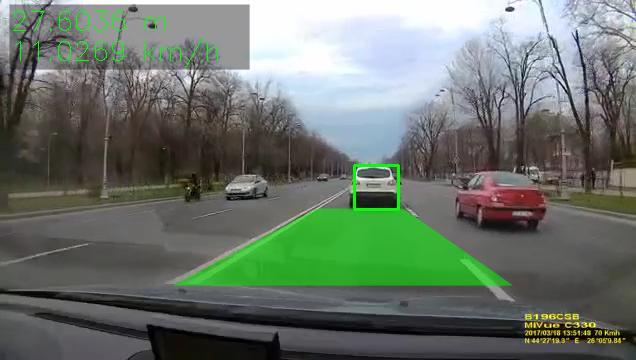
\includegraphics[max width=12cm,max height=12cm,keepaspectratio]{img_1_2}
	\caption[Acoperire sistem Tesla Autopilot]{Acoperire sistem Tesla Autopilot. Imagine preluată din \hyperlink{TeslaAutopilotSystem}{[16]}.}
\end{figure} 

\subsubsection{Waymo}

Autovehicolele Waymo sunt dotate cu senzori și sisteme capabile să detecteze zonele pietonale, bicicliști, alte autovehicole și multe altele pe distanțe similare cu a două terenuri de fotbal. \hyperlink{WaymoSystem}{[20]}

\begin{figure}[!h]
	\centering
	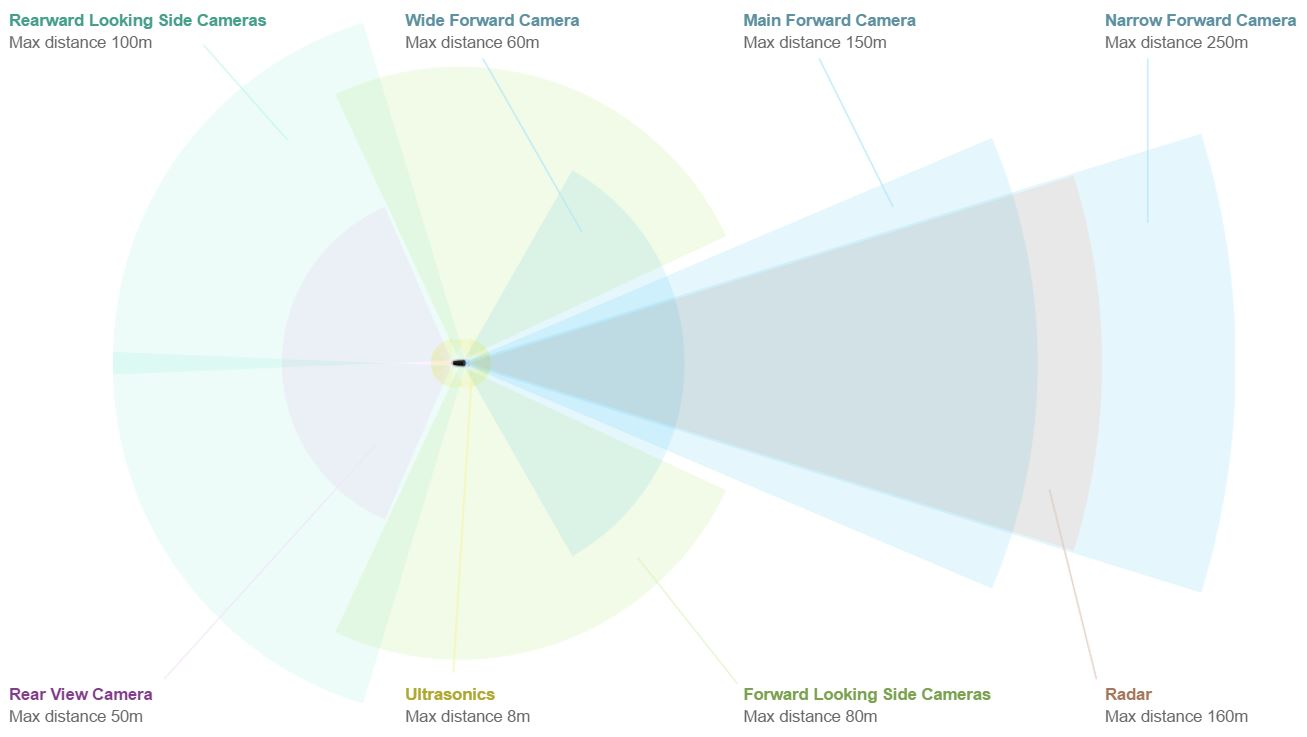
\includegraphics[max width=12cm,max height=12cm,keepaspectratio]{img_1_3}
	\caption[Sistem Waymo]{Sistem Waymo. Imagine preluată din \hyperlink{WaymoSystem}{[20]}.}
\end{figure} 

\section{Structura lucrării}

Prezentarea aplicației realizate debutează prin detalierea fundamentelor teoretice în capitolului II. Aici sunt menționate fundamentele teoretice ce stau la baza realizării acestei prezentei lucrări. 
Capitolul se deschide prin prezentarea noțiunilor despre mașini cu vector suport, un element esențial în antrenarea detectorului de mașini. Pe parcursul acestui capitol prezentăm noțiunile generale despre mașinile cu vector suport, noțiuni despre mașinile cu vector suport multiclasă dar și despre mașinile cu vector suport pentru regresie.

Continuăm prin a descrie histogramele de gradienți orientați folosite în extragerea de caracteristici din imagini. Aceste caracteristici sunt trimise mașinilor cu vectori suport pentru antrenarea dar sunt folosite ulterior și pentru testarea și validarea potențialelor zone ce conțin mașini. 
Se prezintă pe lângă noțiunile generale și etapele algoritmului de extragere a caracteristicilor prin această metodă. 

Metoda glisării ferestrei este și ea abordată în fundamentarea teoretică, această metodă este cea care sta la baza identificării zonelor din imagine pentru care detectorul produce scoruri pozitive în ceea ce privește detecția de autovehicole.

În finalul acestui capitol este prezentată noțiunea de IPM, noțiune esențială în detectarea benzii de circulație, pe de o parte, dar și în analiza datelor privind distanța față de autovehicolul aflăt pe banda curentă și de viteza relativă a acestuia în maniera abordată de lucrare de față.

Capitolul III este dedicat procesului propriu-zis de dezvoltare al aplicației. Începe prin prezentarea componentei ce se ocupă de detectarea benzi. Continuăm prin prezentarea componentei care determină pozițiile eventualelor autovehicole din imagini și vom incheia prin prezentarea metodelor abordate de detectare a distanței față de autovehicolul din față pe banda curentă de circulație împreună cu viteza relativă în raport cu ea.

Spre finalul lucrării, în capitolul IV, vor fi prezentate bazele de date utilizate atât în cadrul componentei ce se ocupă de detectarea benzii de circulație cât și a componentei ce se ocupă de detectarea de autovehicole. Pentru fiecare dintre acestea vor fi prezentate informații generale despre respectiva bază de date, tipurile de imagini pe care le conține, algoritmii de evaluare utilizați pentru validarea rezultatelor obținute, dar și rezultatele propriu-zise.

În închierea lucrării vor fi trase concluziile finale și vor fi prezentate posibile viitoare direcții de dezvoltare ale curentei aplicații.